\chapter{Degrees, counting and proof}
\section*{An odd fact about handshakes}
If everyone at a gathering shakes hands with some of the others, can exactly one person have shaken hands with an odd number of people? The answer is no, and the reason is one of the simplest and most useful graph proofs.

\begin{definition}
The \emph{degree} $\degG(v)$ of a vertex $v$ is the number of edges incident with it, counting parallel edges separately and each loop twice. A vertex of degree 0 is isolated. A vertex adjacent to every other vertex is universal. A vertex is \emph{odd} if its degree is odd, and \emph{even} otherwise.
\end{definition}

\begin{figure}[htbp]
\centering
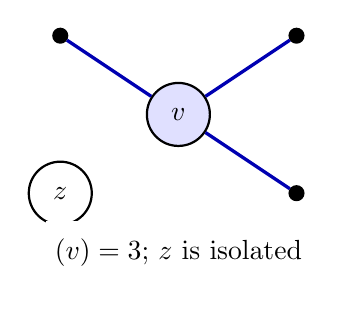
\begin{tikzpicture}[thick,every node/.style={circle,draw,fill=white,minimum size=8mm}]
\node[fill=blue!12] (v) at (0,0) {$v$};
\node[circle,draw=black,fill=black,inner sep=0pt,minimum size=5pt] (a) at (-1.5,1) {};
\node[circle,draw=black,fill=black,inner sep=0pt,minimum size=5pt] (b) at (1.5,1) {};
\node[circle,draw=black,fill=black,inner sep=0pt,minimum size=5pt] (c) at (1.5,-1) {};
\node (z) at (-1.5,-1) {$z$};
\draw[blue!70!black,line width=1.2pt] (v)--(a) (v)--(b) (v)--(c);
\node[draw=none,rectangle] at (0,-1.75) {$\degG(v)=3$; $z$ is isolated};
\end{tikzpicture}
\caption{The degree counts the edges incident with a vertex.}
\end{figure}

\begin{theorem}[\Core{} Handshaking lemma]
For any finite undirected graph, $\sum_{v\in V}\degG(v)=2|E|$.
\end{theorem}
\begin{figure}[htbp]
\centering
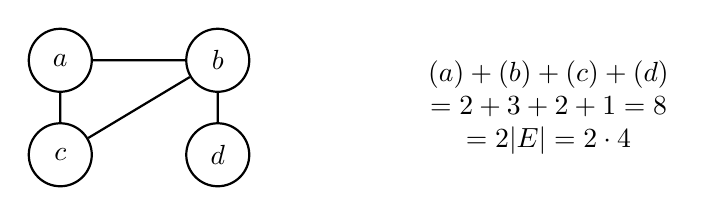
\begin{tikzpicture}[thick,every node/.style={circle,draw,fill=white,minimum size=8mm}]
\node (a) at (0,1.2) {$a$}; \node (b) at (2,1.2) {$b$};
\node (c) at (0,0) {$c$}; \node (d) at (2,0) {$d$};
\draw (a)--(b) (a)--(c) (b)--(c) (b)--(d);
\node[draw=none,rectangle,align=center] at (6.2,0.6) {$\degG(a)+\degG(b)+\degG(c)+\degG(d)$\\$=2+3+2+1=8$\\$=2|E|=2\cdot4$};
\end{tikzpicture}
\caption{Each edge contributes one incidence at each of its two endpoints.}
\end{figure}
\begin{proof}
Count endpoint-incidences, where each incidence pairs an edge with one of its two endpoint occurrences. Each edge contributes two incidences, including a loop, whose two incidences are with the same vertex. Counting instead by vertex, vertex $v$ contributes $\degG(v)$ incidences. These are two counts of the same set, hence the equality.
\end{proof}

\begin{corollary}
Every finite undirected graph has an even number of odd-degree vertices.
\end{corollary}
\begin{figure}[htbp]
\centering
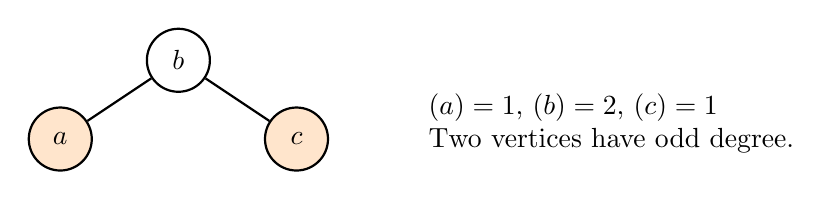
\begin{tikzpicture}[thick,every node/.style={circle,draw,fill=white,minimum size=8mm}]
\node[fill=orange!20] (a) at (0,0) {$a$};
\node[fill=white] (b) at (1.5,1) {$b$};
\node[fill=orange!20] (c) at (3,0) {$c$};
\draw (a)--(b)--(c);
\node[draw=none,rectangle,align=left] at (7,0.2) {$\degG(a)=1$, $\degG(b)=2$, $\degG(c)=1$\\Two vertices have odd degree.};
\end{tikzpicture}
\caption{Odd-degree vertices occur in pairs (here, the two orange endpoints).}
\end{figure}
\begin{proof}
The sum of all degrees is even by the handshaking lemma. A sum of integers is even precisely when it contains an even number of odd summands. Therefore the number of odd-degree vertices is even.
\end{proof}

\begin{definition}
The complete graph $K_n$ has $n$ vertices and an edge between every pair of distinct vertices. A graph is \emph{bipartite} if its vertices can be divided into two sets so every edge joins one set to the other. The cycle graph $C_n$ is a single cycle on $n$ vertices.
\end{definition}

\begin{figure}[htbp]
\centering
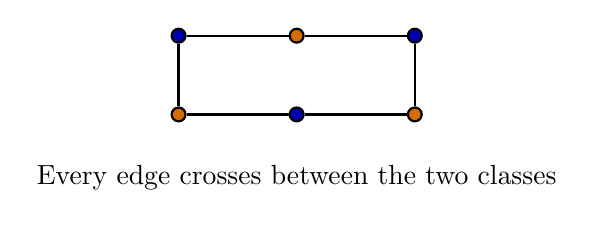
\begin{tikzpicture}[thick,vertex/.style={circle,draw=black,fill=black,inner sep=0pt,minimum size=5pt}]
\node[vertex,fill=blue!70!black] (a) at (0,1) {};
\node[vertex,fill=orange!85!black] (b) at (1.5,1) {};
\node[vertex,fill=blue!70!black] (c) at (3,1) {};
\node[vertex,fill=orange!85!black] (d) at (3,0) {};
\node[vertex,fill=blue!70!black] (e) at (1.5,0) {};
\node[vertex,fill=orange!85!black] (f) at (0,0) {};
\draw (a)--(b)--(c)--(d)--(e)--(f)--(a);
\node[draw=none,rectangle,fill=white] at (1.5,-0.8) {Every edge crosses between the two classes};
\end{tikzpicture}
\caption{The even cycle $C_6$ is bipartite: adjacent vertices have opposite colours.}
\end{figure}

In $K_n$, each vertex has degree $n-1$. Thus $2|E|=n(n-1)$ and $|E|=\binom n2$. The complete bipartite graph $K_{r,s}$ has $r+s$ vertices and $rs$ edges.

\begin{example}
A graph has degree sequence $3,3,2,2,2$. The sum is 12, so it has 6 edges. A proposed degree sequence $3,3,3,1$ cannot describe a graph: it has three odd entries, contradicting the corollary.
\end{example}

A counterexample is often the shortest way to disprove a universal claim. For instance, ``every graph with an even number of vertices has an even number of edges'' fails for a triangle together with an isolated vertex: four vertices, three edges.

\begin{theorem}[\Challenge{} A degree-sum test for connectedness]
Let $G$ be a finite simple graph on $n\geq 1$ vertices. If every pair of nonadjacent vertices $u,v$ satisfies $\degG(u)+\degG(v)\geq n-1$, then $G$ is connected; in fact, any two vertices are at distance at most 2.
\end{theorem}
\begin{proof}
Take any two distinct vertices $u,v$. If they are adjacent, they are joined by a path of length 1. Otherwise, let $N(u)$ and $N(v)$ be their sets of neighbours; both lie among the other $n-2$ vertices. Since
\[
|N(u)|+|N(v)|=\degG(u)+\degG(v)\geq n-1>n-2,
\]
the two neighbour sets must overlap. A common neighbour gives a path of length 2 from $u$ to $v$. Thus every pair is joined by a path of length at most 2.
\end{proof}

\Enrichment{} \textbf{Havel--Hakimi reduction.} To test a nonincreasing sequence of nonnegative integers, remove its largest term $d$ and subtract 1 from the next $d$ terms, then reorder. The Havel--Hakimi theorem says the original sequence is graphical exactly when this process reaches the all-zero sequence; a negative term or too few remaining terms makes it non-graphical.

\section*{Exercises}
\begin{enumerate}
\item Prove that in any simple graph on $n$ vertices, every degree is at most $n-1$.
\item How many edges are in $K_{12}$ and in $K_{4,7}$?
\item A graph has 9 edges. Can all its vertices have degree 3? If so, how many vertices must it have?
\item Disprove: ``If a graph has an even number of edges, then every vertex has even degree.''
\item \Challenge{} The Petersen graph has 10 vertices, each of degree 3. Use the handshaking lemma to find its number of edges.
\item \Enrichment{} Apply the Havel--Hakimi reduction to the sequence $3,3,2,2,2$. (a) Remove the largest term and reduce the next terms as prescribed; reorder the result. (b) Repeat until you reach zeros or detect that the sequence is not graphical. (c) Starting from the last reduction, reverse your steps to construct a graph with the original degree sequence, then check its degrees. (d) Try the same test on $3,3,1,1$. At which step does it fail?
\end{enumerate}
